
% Preamble
% ---
\documentclass{article}

% Packages
% ---
\usepackage{amsmath} % Advanced math typesetting
\usepackage[utf8]{inputenc}
\usepackage{polski}
\usepackage[polish]{babel}
\usepackage{hyperref} % Add a link to your document
\usepackage{graphicx} % Add pictures to your document
\usepackage{listings} % Source code formatting and highlighting
\usepackage{xcolor}
\usepackage{float}
\lstset { %
	language=C++,
	backgroundcolor=\color{black!5}, % set backgroundcolor
	basicstyle=\footnotesize,% basic font setting
}
\graphicspath{{obrazy/}}

\begin{document}
% Set up the maketitle command
\author{Joanna Lebica, Piotr Olbrot}
\title{Klasyfikacja zespołów QRS z użyciem metody SVM RBF}
\date{2017} % You can remove \today{} and type a date manually

\maketitle{} % Generates title

\tableofcontents{} % Generates table of contents from sections
\section {Wstęp}
Od wielu lat, tematyka automatycznej klasyfikacji elektrokardiogramu jest wnikliwie badana przez wiele zespołów. Wynika to z faktu, że pozwala uzyskać użyteczne informacje dotyczące rytmu oraz funkcjonowania serca. Analiza sygnału elektrokardiograficznego jest uważana za skuteczną metodę diagnostyczną w stanach chorobowych układu sercowonaczyniowego. 

W ostatnich latach stosuje się coraz bardziej wyrafinowane metody klasyfikacji, do których zaliczają się m.in. która integrują w sobie elementy logiki rozmytej, sieci neuronowych, ukrytych modeli Markowa, transformacji falkowej oraz maszyny wektorów nośnych.

Jednym z kluczowych aspektów projektu systemu automatycznej klasyfikacji jest właśnie dobór metody klasyfikacji. Metoda SVM jest warta uwagi, ponieważ oparta jest na maksymalizacji obszaru pomiędzy hiperpłaszczyznami rozdzielającymi dane z dwóch grup. Znalazła ona zastosowanie w dziedzinach rozpoznawania obiektów 3-D, obrazowania medycznego i kompresji obrazów. \cite{melgani}

\section{Zarys proponowanego rozwiązania}

Rozwiązanie stworzone w ramach projektu składa się z następujących elementów

\begin{itemize}
	\item{Pobranie sygnału EKG z bazy danych MIT-BIH Arrhythmia Database}
	\item{Wstępne przetworzenie sygnału polegające na filtracji pasmowoprzepustowej oraz odjęciu linii izoelektrycznej}
	\item{Wyznaczenie przybliżonych miejsc występowania zespołów QRS na podstawie pliku .atr dołączonego każdego z badań}
	\item{Dla każdego z zespołów, które zostały sklasyfikowane jako normalny - N lub komorowy - V wyznaczenie cech sygnału}
	\item{Stworzenie macierzy zawierającej w kolejnych wierszach zestawy cech dotyczącej każdego z zespołów QRS, w ostatniej kolumnie informacja o poprawnym przyporządkowaniu (wartość +1 dla N, wartość -1 dla V)}
	\item{Stworzenie zbioru uczącego i testowego}
	\item{Uczenie modelu maszyny wektorów nośnych przy użyciu algorytmu sequential minimal optimization}
	\item{Walidacja modelu z użyciem zbioru testowego}
\end{itemize}

\section{Obliczenie cech kompleksów QRS}

Podawanie do algorytmu uczącego całego sygnału bądź też interesujących fragmentów byłoby niepraktyczne z racji dużej złożoności obliczeniowej takiego rozwiązania. Znalezienie prostych do obliczenia cech zespołów QRS, które jednocześnie są w stanie pogrupować dane wejściowe według rodzaju ewolucji serca byłoby najbardziej korzystną sytuacją. \cite{august}

\subsection{Matematyczny sposób obliczenia cech}
Do analizy wybrano 5 prostych do obliczenia parametrów, do których obliczenia wykorzystuje się fragmenty sygnału uznane jako należące do zespołu QRS. \cite{p15}
Te parametry to:

\begin{itemize}
	\item{Stosunek pola do obwodu (współczynnik Malinowskiej)
	\begin{equation}
	p_1 = \frac{\sum_{k=1}^{N} s[k]}{\sum_{k=2}^{N} s[k]-s[k-1]}
	\end{equation}	}
	\item{Wartość międzyszczytowa
	\begin{equation}
	p_2 = \frac{\max_{k \in <1,N>} s[k]}{\min_{k \in <1,N>} s[k]}
	\end{equation}}
	\item{Procent próbek sygnału, które są ujemne
	\begin{equation}
	p_3 = 100\% * \frac{\sum_{k=1}^{N} u[k]}{N}
	\end{equation} }
	Gdzie:
	\[ u[k] =
	\begin{cases}
	1       & \quad \text{gdy } s[k] < 0\\
	0	    & \quad \text{gdy } s[k] \geq 0\\
	\end{cases}
	\]
	\item{Stosunek maksymalnej prędkości do maksymalnej amplitudy
	\begin{equation}
	p_4 = \frac{\max_{k \in <3,N>} s[k]-s[k-2]+2s[k-1]}{|\max_{k \in <1,N>} s[k] - \min_{k \in <1,N>} s[k]|}
	\end{equation}}
	\item{Stosunek liczby próbek sygnału, których prędkość przekracza 40\% maksymalnej prędkości obserwowanej w sygnale
	\begin{equation}
	p_5 = \frac{\sum_{k=1}^{N} g[k]}{N}
	\end{equation}}
	Gdzie:
	\[ g[k] =
	\begin{cases}
	1       & \quad \text{gdy } |s[k]-s[k-1]| > 0.4 \max_{m \in <2,N>} |s[m]-s[m-1]|\\
	0	    & \quad \text{gdy } |s[k]-s[k-1]| \leq 0.4 \max_{m \in <2,N>} |s[m]-s[m-1]|\\
	\end{cases}
	\]
\end{itemize}
\subsection{Klasyfikacja przy użyciu obliczonych cech}
W celu wstępnej oceny wybranych cech, wybrano losowo 5 sygnałów z bazy danych (100.dat, 107.dat, 114.dat, 200.dat, 208.dat). Wyodrębiono z nich 9306 zespołów QRS, które sklasyfikowano jako normalne (N) bądź komorowe (V). Poniżej przedstawione są wykresy pudełkowe pokazujące zakres zmienności kolejnych cech dla obu grup.

\begin{figure}[H]
	\begin{center}
		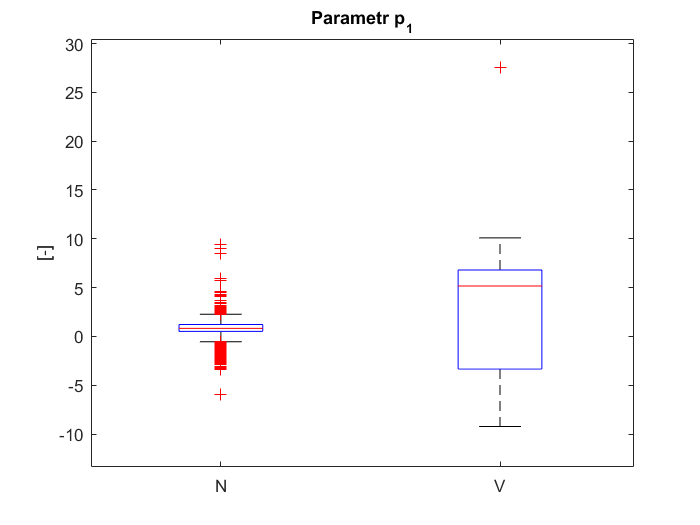
\includegraphics[width=9cm]{p1.png}
		\caption{Parametr $p_1$ dla obu grup}
	\end{center}
\end{figure}

\begin{figure}[H]
	\begin{center}
		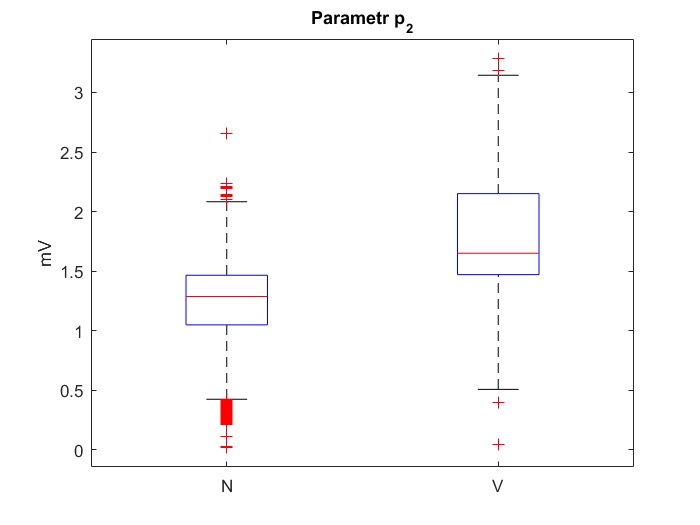
\includegraphics[width=9cm]{p2.png}
		\caption{Parametr $p_2$ dla obu grup}
	\end{center}
\end{figure}

\begin{figure}[H]
	\begin{center}
		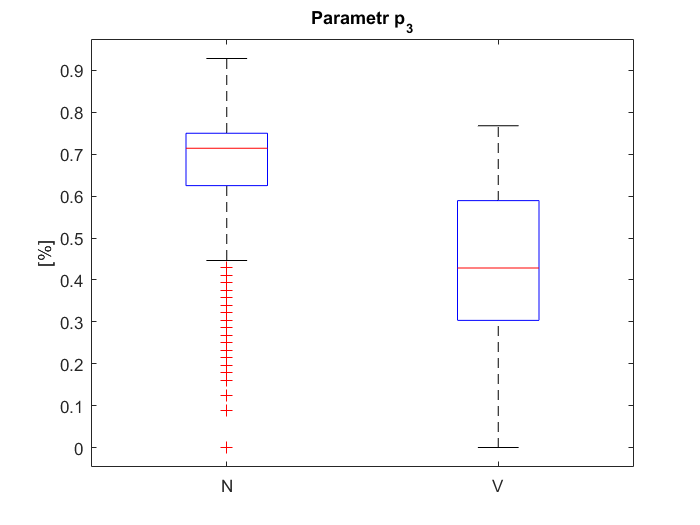
\includegraphics[width=9cm]{p3.png}
		\caption{Parametr $p_3$ dla obu grup}
	\end{center}
\end{figure}

\begin{figure}[H]
	\begin{center}
		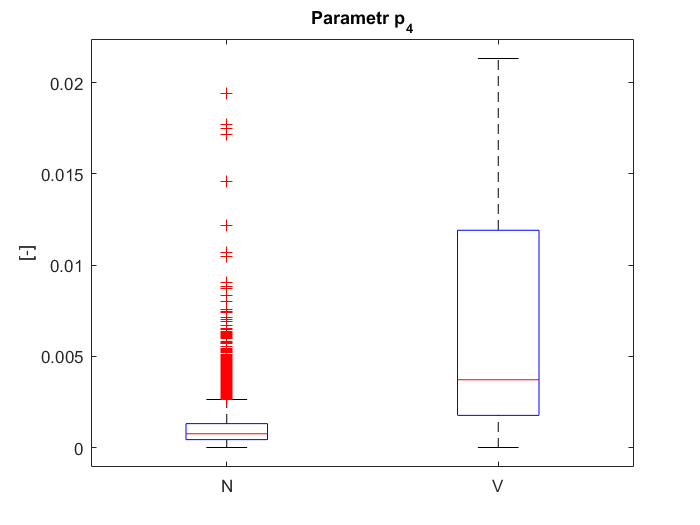
\includegraphics[width=9cm]{p4.png}
		\caption{Parametr $p_4$ dla obu grup}
	\end{center}
\end{figure}

\begin{figure}[H]
	\begin{center}
		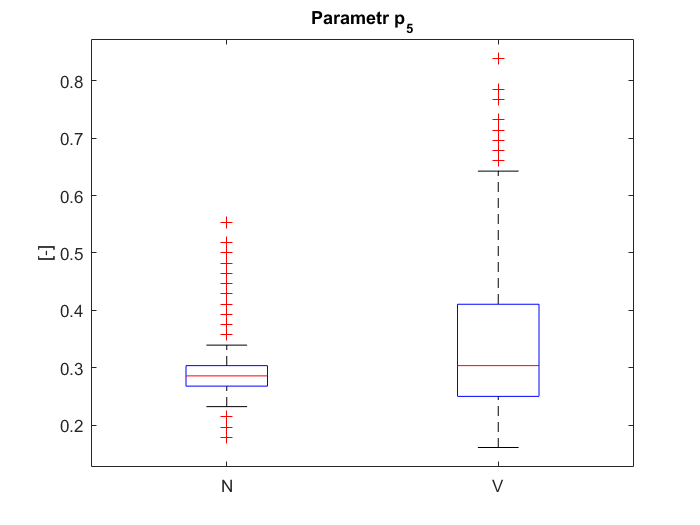
\includegraphics[width=9cm]{p5.png}
		\caption{Parametr $p_5$ dla obu grup}
	\end{center}
\end{figure}

Jak można zauważyć niektóre cechy (przede wszystkim $p_2$ i $p_3$) dobrze dokonują rozróżnienia. W celu potwierdzenia tej obserwacji stworzono wykres obserwacji w przestrzeni $p_2$ - $p_3$.

\begin{figure}[H]
	\begin{center}
		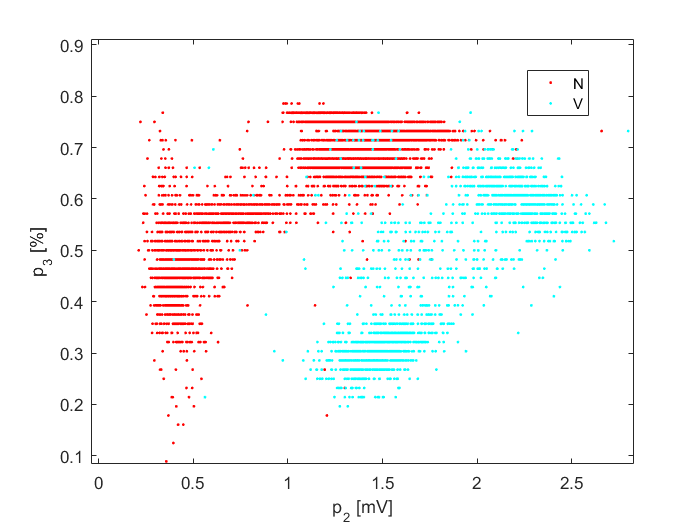
\includegraphics[width=10cm]{p2p3.png}
		\caption{Zbiór testowy na płaszczyźnie $p_2$-$p_3$}
	\end{center}
\end{figure}


Pokazuje on, że klasyfikacja już w przestrzeni tych dwóch cech może dawać satysfakcjonujące rezultaty. Do algorytmu uczącego podano jednak macierz zawierającą wszystkie 5 cech zespołów QRS.
\section{Metoda maszyny wektorów nośnych (SVM)}
\subsection{Podstawowe założenia metody}
Metoda wektorów nośnych dokonuje binarnej (na dwa pozbiory) klasyfikacji z nadzorem. Zbiór uczący składa się z $N$ wektorów
\begin{equation}
x_i \in R^d (i = 1, 2, 3...)
\end{equation}
z $d$-wymiarowej przestrzeni cech $X$. Z każdym wektorem stowarzyszona jest wartość
\begin{equation}
y_i \in \{-1, +1\}
\end{equation}
Metoda SVM w najprostszym (liniowym) wydaniu szuka hiperpłaszczyzny rozdzielającej dwie klasy w przestrzeni $X$ tak, aby hiperpłaszczyzna była najbardziej oddalona od obserwacji zbioru uczącego (maksymalny odstęp).

W przypadku, gdy zbiory nie są liniowo separowalne, obie klasy są wcześniej mapowane do innej przestrzeni cech (o wyższej wymiarowości). Więcej o tym w kolejnym podrozdziale.

Decyzja dotycząca klasyfikacji polega na obliczeniu wartości funkcji dyskryminacyjnej $f(x)$.
\begin{equation}
f(x) = \omega\text{*} \Phi(x) + b\text{*}
\end{equation}
Optymalna hiperpłaszczyzna jest zdefiniowana przez wektor wag
\begin{equation}
\omega\text{*} \in R^{d^\prime}
\end{equation}
i bias
\begin{equation}
b\text{*} \in R
\end{equation}

Optymalizacja klasyfikatora polega na minimalizacji błędu (tj. sumy kar za źle sklasyfikowane obserwacje) oraz maksymalizacji szerokości odległości między hiperpłaszczyzną rozdzielającą a obserwacjami. Przez odpowiedni dobór parametrów można większą wagę postawić na jedną z tych zależności.
\subsection{Radial Basis Function}
Radial Basis Function (lub radialna funkcja bazowa) jest funkcją zależącą jedynie od odległości od pewnego przyjętego środka. Każda funkcja spełniająca warunek
\begin{equation}
\phi(x) = \phi(||x||)
\end{equation}
jest funkcją radialną.

Wprowadzenie radialnej funkcji bazowej związane jest z tym, że w wielu przypadkach niemożliwy jest skuteczny podział w wyjściowej przestrzeni cech. Funkcje bazowe usuwają tę przeszkodę przenosząc problem klasyfikacji do przestrzeni o wyższej wymiarowości, co schematycznie pokazuje poniższy rysunek.

W algorytmie wykonanym w ramach projektu wykorzystano Gaussowską radialną funkcję bazową opisaną wzorem:

\begin{equation}
k(\vec{x}_i,\vec{x}_j) = exp(\frac{||\vec{x}_i-\vec{x}_j||^2}{2\sigma^2})
\end{equation}
\subsection{Wykorzystana metoda implementacji}
\subsubsection{Matematyczne podstawy}

Zastosowana metoda optymalizacji modelu SVM to Sequentual minimal optimization w skrócie SMO. Jest to metoda rozwiązywania zadania optymalizacyjnego polegającego na znalezieniu ekstremum funkcji kwadratowej. Przy implementacji oparto się na opisie z artykułu \cite{svmsmo}. 

SMO jest efektywną metodą rozwiązania problemu optymalizacji, który może być opisany następującym równaniem

\begin{equation}
\max_{\alpha} W(\alpha) = \sum_{i=1}^{m}\alpha_i - \frac{1}{2}\sum_{i=1}^{m}\sum_{j=1}^{m}y^{i}y^{j}\alpha_i\alpha_j\langle x^{(i)},x^{(j)}\rangle
\end{equation}
Gdzie:
\begin{equation}
0\leq \alpha_i \leq C, \text{dla } i = 1, 2, 3, ..., m
\end{equation}
\begin{equation}
	\sum_{i=1}^{m}y^{(i)}\alpha_i=0
\end{equation}
Warunek znalezienia optymalnego rozwiązania (zwany warunkiem Karusha-Kuhna-Tuckera) dla tego problemu jest zdefiniowany następująco
\begin{equation}
\alpha_i = 0 \implies y^{(i)}(\omega^{T}x^{(i)}+b)\geq1
\end{equation}
\begin{equation}
\alpha_i = C \implies y^{(i)}(\omega^{T}x^{(i)}+b)\leq1
\end{equation}
\begin{equation}
0 < \alpha_i < C \implies y^{(i)}(\omega^{T}x^{(i)}+b)= 1
\end{equation}
Algorytm SMO iteruje aż do momentu, gdy te warunki zostaną spełnione przez to zapewniając jego zbieżność do optymalnego rozwiązania.

Składa się on 3 kroków \cite{svmsmo}:
\begin{itemize}
	\item Wybór parametrów $\alpha$
	W zaimplementowanym algorytmie zastosowano najprostszy wybór parametrów, tj. w pętli iteruje się przez wszystkie $\alpha_i$, a następnie losuje się $\alpha_j$ takie, że $i \neq j$. Istnieje niewielkie prawdopodobieństwo, że któraś z par parametrów, które wprowadziłyby istotną zmianę do ostatecznego wyniku zostanie pominięta. Założono jednak, że algorytm musi wykonać przynajmniej 10 (domyślna wartość) "pustych przebiegów", aby zminimalizować takie prawdopodobieństwo. "Pusty przebieg" polega na tym, że w danej iteracji pętli zewnętrznej nie zostają wprowadzone żadne zmiany do modelu.
	\item Optymalizacja $\alpha_i$ i $\alpha_j$
	Obliczane są ograniczenia, które musi spełniać $\alpha_j$, a natępnie rozwiązywany jest ograniczony problem optymalizacyjny. Następnie obliczana jest $\alpha_j$ optymalna dla danego kroku, która jest następnie ogranicza jeśli posiada wartość spoza założonego zakresu. Na podstawie $\alpha_j$ obliczana jest nowa wartość $\alpha_i$. Odpowiednie wzory dostępne są \cite{svmsmo}.
	\item Obliczenie biasu $b$
	Po obliczeniu $\alpha_i$ i $\alpha_j$, wybierana jest taka wartość $b$, żeby warunek znalezienia optymalnego rozwiązania był spełniony. Sprawdzane jest, czy obliczone uprzednio $\alpha_i$ i $\alpha_j$ znajdują się na granicach przedziału $<0,C>$. Jeśli nie, to dane rozwiązanie jest prawidłowe. Jeśli oba nie są na granicach przedziału wartość $b$ jest średnią arytmetyczną $b_1$ i $b_2$ obliczoną odpowiednio dla $\alpha_i$ i $\alpha_j$. Szczegóły: \cite{svmsmo}.
\end{itemize}
\subsubsection{Implementacja w C++}

W przygotowaniu programu w C++ wykorzystano bibliotekę Eigen, która okazała się szczególnie przydatna z racji wbudowanych funkcji obsługujących macierze i wektory. Najważniejsze elementy programu to:
\begin{itemize}
	\item Klasa SVM - jest to klasa obsługująca proces uczenia modelu (metoda train), a następnie jego testowania (metoda predict), posiada szereg funkcji prywatnych funkcji pomocniczych
	\item Funkcja parseData - jest to funkcja odpowiadająca za wczytanie odpowiednio zdefiniowanego pliku CSV i stworzenie na jego podstawie struktury zawierającej 2 macierze (treningową, testową) i 2 wektory (poprawne przyporządkowanie dla zbioru treningowego i testowego)
	\item Funkcje writeDecisionToCSV i appendToOutputFile - odpowiadające za zapis do plików działania modelu
	\item Struktura SVMOptions - zawierający parametry działania metody maszyny wektorów nośnych oraz domyślny konstruktor przyjmujący wartości domyślne
	\item Struktura ParsedData - zawierający całość danych potrzebnych do uczenia i testowania modelu
\end{itemize}

Funkcja główna main zawiera kod wywołujący poszczególne elementy programu:

\begin{lstlisting}
int main(int argc, char** argv){

// wczytaj dane z plikow, ktorych nazwe podano w konsoli
// - zalozono, ze pliki z danymi znajduja sie w tym samym
// folderze co program

ParsedData data = parseData(argv);

// utworz model, podano domyslne parametry tj. C(1.0),
// tol(0.0001), sigma(0.5), iterLimit(10000),
// passLimit(10)

SVM model(data.trainSet, data.trainSetOut, SVMOptions());

// trenuj model na danych podanych w konstruktorze
model.train();

// dokonaj klasyfikacji danych podanych w pliku
// testowym; zapisz wektor z klasyfikacja do pliku CSV o
// nazwie out.csv

VectorXd decision = model.massPredict(data.testSet);
writeDecisionToCSV(decision);

// ocen dzialanie klasyfikatora (ilosc poprawnie
// sklasyfikowanych ewolucji serca N/V) oraz czas
// uczenia i testow

evaluateModel(data.testSetOut, decision);
appendToOutputFile(model.trainTime, model.testTime);

return 0;
}
\end{lstlisting}

\section{Wyniki}
Spośród ponad 9 tysięcy obserwacji do trenowania wybrano losowo 400 (322 zespoły QRS typu N, 76 zespoły typu V, jest to naturalna proporcja w jakiej występowały te zespoły w przebiegach 5 sygnałów, które wybrano losowo z bazy danych), a do testowania 100.

Zbiór uczący pokazano poniżej, w płaszczyźnie $p_1$-$p_2$ (po lewej) i $p_2$-$p_4$ (po prawej).

\begin{figure}[H]
	\begin{center}
		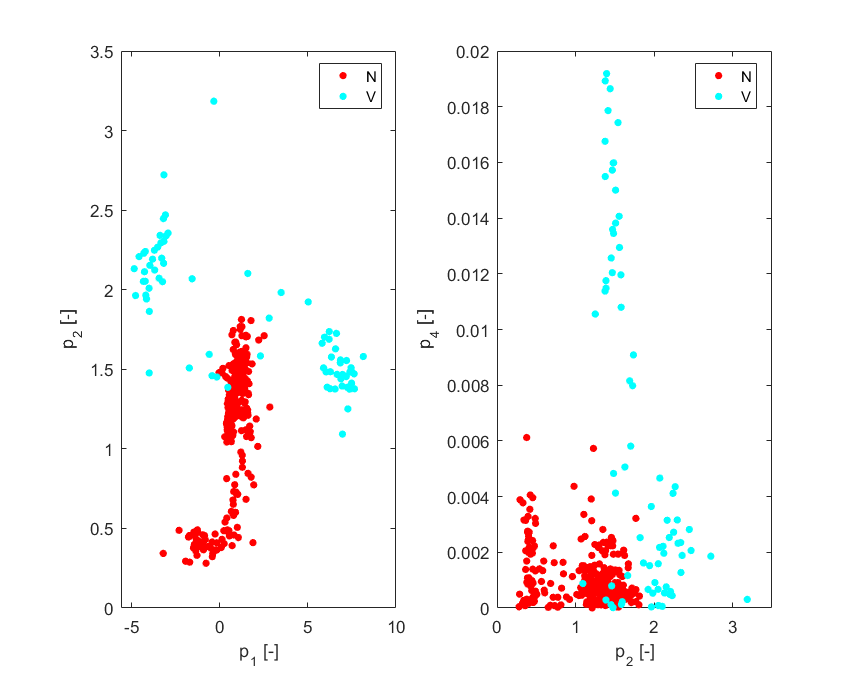
\includegraphics[width=11cm]{trening1.png}
		\caption{Zbiór uczący na płaszczyźnie $p_1$-$p_2$ (po lewej) i $p_2$-$p_4$ (po prawej)}
	\end{center}
\end{figure}


Poniżej zwizualizowano zbiór testowy (n/v) i treningowy (N/V) na jednym wykresie w tych samych płaszczyznach.

\begin{figure}[H]
	\begin{center}
		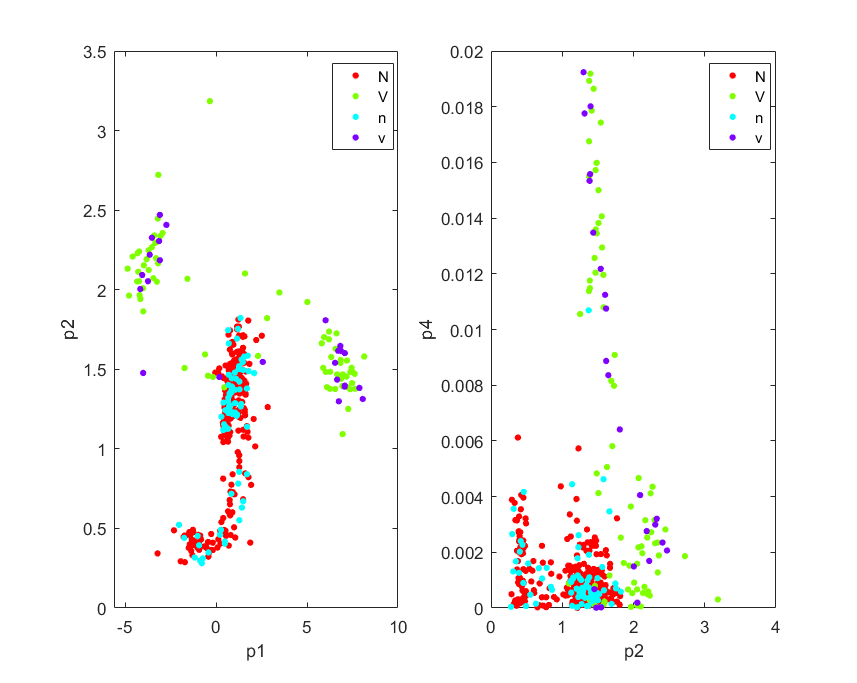
\includegraphics[width=11cm]{treningtest1.png}
		\caption{Zbiór uczący i testowy na płaszczyźnie $p_1$-$p_2$ (po lewej) i $p_2$-$p_4$ (po prawej)}
	\end{center}
\end{figure}


Zaimplementowana metoda klasyfikacji poprawnie przyporządkowała 99 spośród 100 obserwacji. Na wykresie porównawczym (po lewej poprawne przyporządkowanie, po prawej wynik działania algorytmu) oznaczono źle sklasyfikowaną obserwację.

\begin{figure}[H]
	\begin{center}
		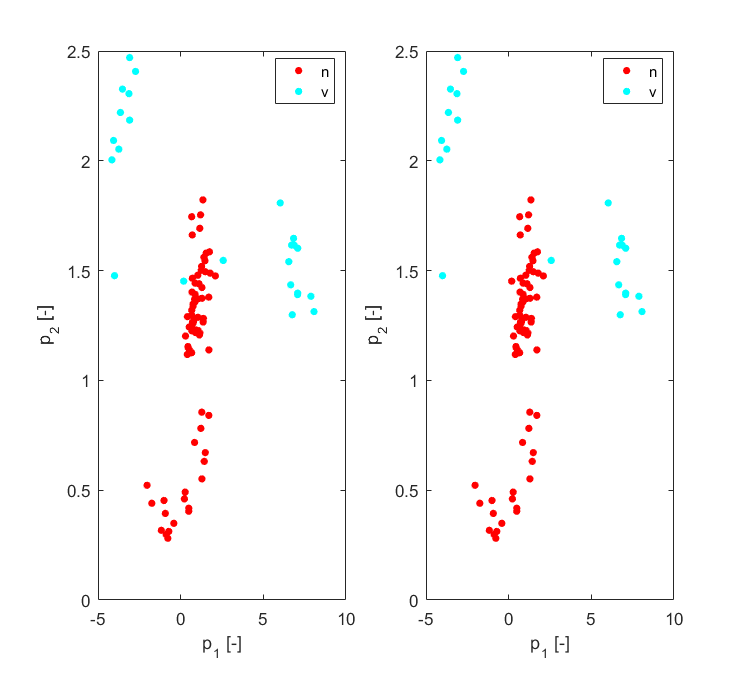
\includegraphics[width=11cm]{testwynik.png}
		\caption{Poprawnie sklasyfikowany zbiór uczący na płaszczyźnie $p_1$-$p_2$ (po lewej) i wynik działania algorytmu w tej samej płaszczyźnie (po prawej)}
	\end{center}
\end{figure}

Porównanie działania algorytmu SVM RBF z algorytmami innych grup znajduje się w osobnym raporcie.

\section{Wnioski}

Klasyfikator zespołów QRS stworzony w ramach projektu działa satysfakcjonująco dla wybranych cech fragmentów sygnału i zaimplementowanego algorytmu SVM.

W ramach projektu wykorzystano sprawdzone, ale proste matematycznie parametry sygnału i potwierdziły one swoją zdolność do rozróżniania zespołów QRS o różnym pochodzeniu pobudzenia. W ramach projektu porównywano zespoły sklasyfikowane jako normalne (N) oraz komorowe (V). Należy przyjąć, że gdyby dokonano bardziej szczegółówego podziału działanie klasyfikatora uległoby pogorszeniu. Już w początkowej fazie projektu stwierdzono, że bardzo ciężko byłoby odróżnić zespoły normalne (N) od nadkomorowych (SV) wg klasyfikacji. \cite{survey}

Spośród wszystkich metod SVM realizowanych w projekcie metoda SVM RBF zapewnia najlepszą skuteczność rozdziału cech, która w przestrzeni, w której są zdefiniowane nie są liniowo separowalne, co stanowi niewątpliwą zaletę tego algorytmu. \cite{melgani}

Czas trenowania klasyfikatora tj. ok. 20 sekund (na komputerze jednego z autorów) dla 400 obserwacji po 5 cech każda można uznać za zadowalający, ale z pewnością istnieje wiele metod dalszej optymalizacji kodu.

\begin{thebibliography}{9}
	
	\bibitem{melgani}
	Bazi Yakoub, Melgani Farid
	\textit{Classification of Electrocardiogram Signals With Support Vector Machines and Particle Swarm Optimization} 
	IEEE Transactions on Information Technology in Biomedicine 12, 2008
	\bibitem{survey}
	da Luza E. J. S, et al.
	\textit{ECG-based Heartbeat Classification for Arrhytmia Detection: A Survey} 
	Computer methods and programs in biomedicine, 2016
	\bibitem{august}
	Augustyniak Piotr
	\textit{Przetwarzanie sygnałów elektrodiagnostycznych} 
	Wydawnictwa AGH, Kraków, Poland, 2001
	\bibitem{svmsmo}
	Husanbir Singh Pannu
	\textit{Simplified SMO Algorithm} 
	\\\texttt{http://math.unt.edu/~hsp0009/smo.pdf}
	\bibitem{p15} 
	Augustyniak Piotr
	\textit{Optymalizacja wyboru reprezentacji zespołów skurczowych dla celów klasyfikacji zapisów holterowskich} 
	\\\texttt{http://galaxy.uci.agh.edu.pl/~august/pub/pdf/p15.pdf}
	
\end{thebibliography}
%\bibliographystyle{unsrt}
%\bibliography{biblio}

\end{document}